% Options for packages loaded elsewhere
\PassOptionsToPackage{unicode}{hyperref}
\PassOptionsToPackage{hyphens}{url}
%
\documentclass[
]{article}
\usepackage{lmodern}
\usepackage{amssymb,amsmath}
\usepackage{ifxetex,ifluatex}
\ifnum 0\ifxetex 1\fi\ifluatex 1\fi=0 % if pdftex
  \usepackage[T1]{fontenc}
  \usepackage[utf8]{inputenc}
  \usepackage{textcomp} % provide euro and other symbols
\else % if luatex or xetex
  \usepackage{unicode-math}
  \defaultfontfeatures{Scale=MatchLowercase}
  \defaultfontfeatures[\rmfamily]{Ligatures=TeX,Scale=1}
\fi
% Use upquote if available, for straight quotes in verbatim environments
\IfFileExists{upquote.sty}{\usepackage{upquote}}{}
\IfFileExists{microtype.sty}{% use microtype if available
  \usepackage[]{microtype}
  \UseMicrotypeSet[protrusion]{basicmath} % disable protrusion for tt fonts
}{}
\makeatletter
\@ifundefined{KOMAClassName}{% if non-KOMA class
  \IfFileExists{parskip.sty}{%
    \usepackage{parskip}
  }{% else
    \setlength{\parindent}{0pt}
    \setlength{\parskip}{6pt plus 2pt minus 1pt}}
}{% if KOMA class
  \KOMAoptions{parskip=half}}
\makeatother
\usepackage{xcolor}
\IfFileExists{xurl.sty}{\usepackage{xurl}}{} % add URL line breaks if available
\IfFileExists{bookmark.sty}{\usepackage{bookmark}}{\usepackage{hyperref}}
\hypersetup{
  pdftitle={Logistic Regression Ch5},
  pdfauthor={F.A. Barrios Instituto de Neurobiología UNAM},
  hidelinks,
  pdfcreator={LaTeX via pandoc}}
\urlstyle{same} % disable monospaced font for URLs
\usepackage[margin=1in]{geometry}
\usepackage{color}
\usepackage{fancyvrb}
\newcommand{\VerbBar}{|}
\newcommand{\VERB}{\Verb[commandchars=\\\{\}]}
\DefineVerbatimEnvironment{Highlighting}{Verbatim}{commandchars=\\\{\}}
% Add ',fontsize=\small' for more characters per line
\usepackage{framed}
\definecolor{shadecolor}{RGB}{248,248,248}
\newenvironment{Shaded}{\begin{snugshade}}{\end{snugshade}}
\newcommand{\AlertTok}[1]{\textcolor[rgb]{0.94,0.16,0.16}{#1}}
\newcommand{\AnnotationTok}[1]{\textcolor[rgb]{0.56,0.35,0.01}{\textbf{\textit{#1}}}}
\newcommand{\AttributeTok}[1]{\textcolor[rgb]{0.77,0.63,0.00}{#1}}
\newcommand{\BaseNTok}[1]{\textcolor[rgb]{0.00,0.00,0.81}{#1}}
\newcommand{\BuiltInTok}[1]{#1}
\newcommand{\CharTok}[1]{\textcolor[rgb]{0.31,0.60,0.02}{#1}}
\newcommand{\CommentTok}[1]{\textcolor[rgb]{0.56,0.35,0.01}{\textit{#1}}}
\newcommand{\CommentVarTok}[1]{\textcolor[rgb]{0.56,0.35,0.01}{\textbf{\textit{#1}}}}
\newcommand{\ConstantTok}[1]{\textcolor[rgb]{0.00,0.00,0.00}{#1}}
\newcommand{\ControlFlowTok}[1]{\textcolor[rgb]{0.13,0.29,0.53}{\textbf{#1}}}
\newcommand{\DataTypeTok}[1]{\textcolor[rgb]{0.13,0.29,0.53}{#1}}
\newcommand{\DecValTok}[1]{\textcolor[rgb]{0.00,0.00,0.81}{#1}}
\newcommand{\DocumentationTok}[1]{\textcolor[rgb]{0.56,0.35,0.01}{\textbf{\textit{#1}}}}
\newcommand{\ErrorTok}[1]{\textcolor[rgb]{0.64,0.00,0.00}{\textbf{#1}}}
\newcommand{\ExtensionTok}[1]{#1}
\newcommand{\FloatTok}[1]{\textcolor[rgb]{0.00,0.00,0.81}{#1}}
\newcommand{\FunctionTok}[1]{\textcolor[rgb]{0.00,0.00,0.00}{#1}}
\newcommand{\ImportTok}[1]{#1}
\newcommand{\InformationTok}[1]{\textcolor[rgb]{0.56,0.35,0.01}{\textbf{\textit{#1}}}}
\newcommand{\KeywordTok}[1]{\textcolor[rgb]{0.13,0.29,0.53}{\textbf{#1}}}
\newcommand{\NormalTok}[1]{#1}
\newcommand{\OperatorTok}[1]{\textcolor[rgb]{0.81,0.36,0.00}{\textbf{#1}}}
\newcommand{\OtherTok}[1]{\textcolor[rgb]{0.56,0.35,0.01}{#1}}
\newcommand{\PreprocessorTok}[1]{\textcolor[rgb]{0.56,0.35,0.01}{\textit{#1}}}
\newcommand{\RegionMarkerTok}[1]{#1}
\newcommand{\SpecialCharTok}[1]{\textcolor[rgb]{0.00,0.00,0.00}{#1}}
\newcommand{\SpecialStringTok}[1]{\textcolor[rgb]{0.31,0.60,0.02}{#1}}
\newcommand{\StringTok}[1]{\textcolor[rgb]{0.31,0.60,0.02}{#1}}
\newcommand{\VariableTok}[1]{\textcolor[rgb]{0.00,0.00,0.00}{#1}}
\newcommand{\VerbatimStringTok}[1]{\textcolor[rgb]{0.31,0.60,0.02}{#1}}
\newcommand{\WarningTok}[1]{\textcolor[rgb]{0.56,0.35,0.01}{\textbf{\textit{#1}}}}
\usepackage{graphicx,grffile}
\makeatletter
\def\maxwidth{\ifdim\Gin@nat@width>\linewidth\linewidth\else\Gin@nat@width\fi}
\def\maxheight{\ifdim\Gin@nat@height>\textheight\textheight\else\Gin@nat@height\fi}
\makeatother
% Scale images if necessary, so that they will not overflow the page
% margins by default, and it is still possible to overwrite the defaults
% using explicit options in \includegraphics[width, height, ...]{}
\setkeys{Gin}{width=\maxwidth,height=\maxheight,keepaspectratio}
% Set default figure placement to htbp
\makeatletter
\def\fps@figure{htbp}
\makeatother
\setlength{\emergencystretch}{3em} % prevent overfull lines
\providecommand{\tightlist}{%
  \setlength{\itemsep}{0pt}\setlength{\parskip}{0pt}}
\setcounter{secnumdepth}{-\maxdimen} % remove section numbering

\title{Logistic Regression Ch5}
\author{F.A. BarriosInstituto de Neurobiología UNAM}
\date{2020-11-26}

\begin{document}
\maketitle

\begin{Shaded}
\begin{Highlighting}[]
\KeywordTok{library}\NormalTok{(tidyverse)}
\KeywordTok{library}\NormalTok{(emmeans)}
\KeywordTok{library}\NormalTok{(rstatix)}
\KeywordTok{library}\NormalTok{(HSAUR2)}
\KeywordTok{library}\NormalTok{(car)}
\KeywordTok{library}\NormalTok{(effects)}

\KeywordTok{setwd}\NormalTok{(}\StringTok{"~/Dropbox/GitHub/Class2020"}\NormalTok{)}
\NormalTok{wcgs <-}\StringTok{ }\KeywordTok{read_csv}\NormalTok{(}\StringTok{"DataRegressBook/Chap2/wcgs.csv"}\NormalTok{)}
\end{Highlighting}
\end{Shaded}

\hypertarget{logistic-regression}{%
\section{Logistic Regression}\label{logistic-regression}}

\hypertarget{example-from-hsaur-chapter-7-in-hsaur3}{%
\subsection{Example from HSAUR (Chapter 7, in
HSAUR3)}\label{example-from-hsaur-chapter-7-in-hsaur3}}

\hypertarget{introduction}{%
\subsubsection{Introduction}\label{introduction}}

The erythrocyte sedimentation rate (ESR) is the rate at which red blood
cells (erythrocytes) settle out of suspension in the blood plasma, when
measured under standard conditions. If the ESR increases when the level
of certain proteins in the blood plasma rise in association with
conditions such as rheumatic diseases, chronic infections, and malignant
diseases, its determination might be useful in screening blood samples
taken from people suspected of suffering from one of the conditions
mentioned. The absolute value of the ESR is not of great importance;
rather, less than 20mm/hr indicates a `healthy' individual. To asses
whether the ESR is a useful diagnostic tool, Collett and Jemain (1985)
collected the data in HSAUR2. The question of interest is whether there
is any association between the probability of an ESR reading greater
than 20mm/hr and the levels of the two plasma proteins. If there is not
then the determination of ESR would not be useful for diagnostic
purposes.

\begin{Shaded}
\begin{Highlighting}[]
\CommentTok{# Using plasma data from HSAUR}
\KeywordTok{data}\NormalTok{(}\StringTok{"plasma"}\NormalTok{, }\DataTypeTok{package =} \StringTok{"HSAUR2"}\NormalTok{)}
\KeywordTok{layout}\NormalTok{(}\KeywordTok{matrix}\NormalTok{(}\DecValTok{1}\OperatorTok{:}\DecValTok{2}\NormalTok{, }\DataTypeTok{ncol =} \DecValTok{2}\NormalTok{))}
\CommentTok{# cdplot computes and plots conditional densities describing how the conditional distribution of a categorical variable y changes over a numerical variable x}
\KeywordTok{cdplot}\NormalTok{(ESR }\OperatorTok{~}\StringTok{ }\NormalTok{fibrinogen, }\DataTypeTok{data =}\NormalTok{ plasma)}
\KeywordTok{cdplot}\NormalTok{(ESR }\OperatorTok{~}\StringTok{ }\NormalTok{globulin, }\DataTypeTok{data =}\NormalTok{ plasma)}
\end{Highlighting}
\end{Shaded}

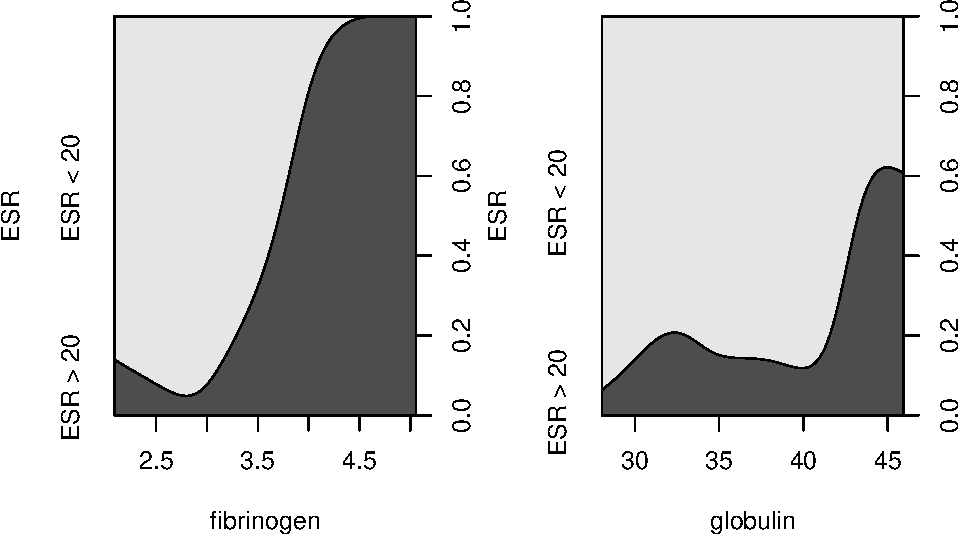
\includegraphics{LogisticRegressionCh5_files/figure-latex/unnamed-chunk-2-1.pdf}
To estimate a logistic regression model in R the glm (General Linear
Model) is used, for binomial distribution the glm() function defalut to
a logistic model.

\begin{Shaded}
\begin{Highlighting}[]
\CommentTok{# glm general linear model default is logistic for binomial distribution}

\NormalTok{plasma_glm01 <-}\StringTok{ }\KeywordTok{glm}\NormalTok{(ESR }\OperatorTok{~}\StringTok{ }\NormalTok{fibrinogen, }\DataTypeTok{data =}\NormalTok{ plasma, }\DataTypeTok{family =} \KeywordTok{binomial}\NormalTok{())}
\KeywordTok{S}\NormalTok{(plasma_glm01)}
\end{Highlighting}
\end{Shaded}

\begin{verbatim}
Call: glm(formula = ESR ~ fibrinogen, family = binomial(), data = plasma)

Coefficients:
            Estimate Std. Error z value Pr(>|z|)  
(Intercept)  -6.8451     2.7703  -2.471   0.0135 *
fibrinogen    1.8271     0.9009   2.028   0.0425 *
---
Signif. codes:  0 '***' 0.001 '**' 0.01 '*' 0.05 '.' 0.1 ' ' 1

(Dispersion parameter for binomial family taken to be 1)

    Null deviance: 30.885  on 31  degrees of freedom
Residual deviance: 24.840  on 30  degrees of freedom

logLik     df    AIC    BIC 
-12.42      2  28.84  31.77 

Number of Fisher Scoring iterations: 5

Exponentiated Coefficients and Confidence Bounds
               Estimate        2.5 %      97.5 %
(Intercept) 0.001064686 1.172299e-06  0.09755943
fibrinogen  6.215715449 1.403209e+00 54.51588384
\end{verbatim}

From these results we see that the regression coefficients for
fibrinogen is significant at the 5\% level. An increase of one unit in
this variable increases the log-odds on favor of an ESR value greater
then 20 by estimated 1.83 with 95\% confidence interval:

\begin{Shaded}
\begin{Highlighting}[]
\CommentTok{# coeff fibrinogen is sifnificative 5%}
\CommentTok{# one unit change in this variable increases the log-odds in favor of ESR > 20mm/hr by 1.83}
\KeywordTok{Confint}\NormalTok{(plasma_glm01, }\DataTypeTok{parm =} \StringTok{"fibrinogen"}\NormalTok{)}
\end{Highlighting}
\end{Shaded}

\begin{verbatim}
             Estimate    result
(Intercept) -6.845075 0.3387619
fibrinogen   1.827081 3.9984921
\end{verbatim}

\begin{Shaded}
\begin{Highlighting}[]
\KeywordTok{exp}\NormalTok{(}\KeywordTok{coef}\NormalTok{(plasma_glm01)[}\StringTok{"fibrinogen"}\NormalTok{])}
\end{Highlighting}
\end{Shaded}

\begin{verbatim}
fibrinogen 
  6.215715 
\end{verbatim}

\begin{Shaded}
\begin{Highlighting}[]
\KeywordTok{exp}\NormalTok{(}\KeywordTok{confint}\NormalTok{(plasma_glm01, }\DataTypeTok{parm =} \StringTok{"fibrinogen"}\NormalTok{))}
\end{Highlighting}
\end{Shaded}

\begin{verbatim}
    2.5 %    97.5 % 
 1.403209 54.515884 
\end{verbatim}

These are the values of the odds themselves (by exponentiating the
estimate). So \textbf{increased values of fibrinogen lead to a grater
probability of an ESR value greater than 20}.

\begin{Shaded}
\begin{Highlighting}[]
\CommentTok{# full model with two variables}
\NormalTok{plasma_glm02 <-}\StringTok{ }\KeywordTok{glm}\NormalTok{(ESR }\OperatorTok{~}\StringTok{ }\NormalTok{fibrinogen }\OperatorTok{+}\StringTok{ }\NormalTok{globulin, }\DataTypeTok{data =}\NormalTok{ plasma, }\DataTypeTok{family =} \KeywordTok{binomial}\NormalTok{())}
\KeywordTok{S}\NormalTok{(plasma_glm02)}
\end{Highlighting}
\end{Shaded}

\begin{verbatim}
Call: glm(formula = ESR ~ fibrinogen + globulin, family = binomial(), data =
          plasma)

Coefficients:
            Estimate Std. Error z value Pr(>|z|)  
(Intercept) -12.7921     5.7963  -2.207   0.0273 *
fibrinogen    1.9104     0.9710   1.967   0.0491 *
globulin      0.1558     0.1195   1.303   0.1925  
---
Signif. codes:  0 '***' 0.001 '**' 0.01 '*' 0.05 '.' 0.1 ' ' 1

(Dispersion parameter for binomial family taken to be 1)

    Null deviance: 30.885  on 31  degrees of freedom
Residual deviance: 22.971  on 29  degrees of freedom

logLik     df    AIC    BIC 
-11.49      3  28.97  33.37 

Number of Fisher Scoring iterations: 5

Exponentiated Coefficients and Confidence Bounds
                Estimate        2.5 %      97.5 %
(Intercept) 2.782735e-06 1.420825e-12  0.04286868
fibrinogen  6.755579e+00 1.404131e+00 73.00083593
globulin    1.168567e+00 9.359678e-01  1.53212986
\end{verbatim}

Comparing the residual deviance of the models: residual deviance 01:
24.84 residual deviance 02: 22.971 -\textgreater{} 1.869 (1.87), to test
for significance R take the lgm with a \(\chi^2\) the 1.87 we conclude
that \textbf{the globulin has no influence in the ESR}. To compare the
two nested models (with fibrinogen and fibrinogen + gamma globulin) we
can estimate the ANOVA of the models (Pr of 0.1716)

\begin{Shaded}
\begin{Highlighting}[]
\KeywordTok{anova}\NormalTok{(plasma_glm01, plasma_glm02, }\DataTypeTok{test =} \StringTok{"Chisq"}\NormalTok{)}
\end{Highlighting}
\end{Shaded}

\begin{verbatim}
Analysis of Deviance Table

Model 1: ESR ~ fibrinogen
Model 2: ESR ~ fibrinogen + globulin
  Resid. Df Resid. Dev Df Deviance Pr(>Chi)
1        30     24.840                     
2        29     22.971  1   1.8692   0.1716
\end{verbatim}

\begin{Shaded}
\begin{Highlighting}[]
\KeywordTok{Anova}\NormalTok{(plasma_glm01)}
\end{Highlighting}
\end{Shaded}

\begin{verbatim}
Analysis of Deviance Table (Type II tests)

Response: ESR
           LR Chisq Df Pr(>Chisq)  
fibrinogen   6.0446  1    0.01395 *
---
Signif. codes:  0 '***' 0.001 '**' 0.01 '*' 0.05 '.' 0.1 ' ' 1
\end{verbatim}

\begin{Shaded}
\begin{Highlighting}[]
\CommentTok{# Estimates conditional probability of a ESR > 20 for all observations}

\NormalTok{prob <-}\StringTok{ }\KeywordTok{predict}\NormalTok{(plasma_glm02, }\DataTypeTok{type =} \StringTok{"response"}\NormalTok{)}
\KeywordTok{layout}\NormalTok{(}\KeywordTok{matrix}\NormalTok{(}\DecValTok{1}\OperatorTok{:}\DecValTok{1}\NormalTok{, }\DataTypeTok{ncol =} \DecValTok{1}\NormalTok{))}

\KeywordTok{plot}\NormalTok{(globulin }\OperatorTok{~}\StringTok{ }\NormalTok{fibrinogen, }\DataTypeTok{data =}\NormalTok{ plasma, }\DataTypeTok{xlim =} \KeywordTok{c}\NormalTok{(}\DecValTok{2}\NormalTok{, }\DecValTok{6}\NormalTok{), }\DataTypeTok{ylim =} \KeywordTok{c}\NormalTok{(}\DecValTok{25}\NormalTok{, }\DecValTok{55}\NormalTok{), }\DataTypeTok{pch =} \StringTok{"."}\NormalTok{)}
\KeywordTok{symbols}\NormalTok{(plasma}\OperatorTok{$}\NormalTok{fibrinogen, plasma}\OperatorTok{$}\NormalTok{globulin, }\DataTypeTok{circles =}\NormalTok{ prob, }\DataTypeTok{add =} \OtherTok{TRUE}\NormalTok{)}
\end{Highlighting}
\end{Shaded}

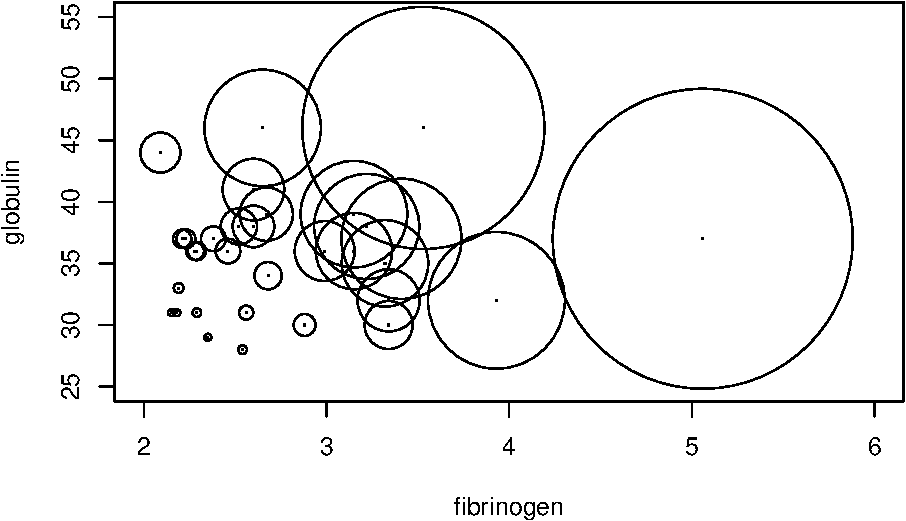
\includegraphics{LogisticRegressionCh5_files/figure-latex/unnamed-chunk-6-1.pdf}

\begin{Shaded}
\begin{Highlighting}[]
\KeywordTok{plot}\NormalTok{(}\KeywordTok{predictorEffects}\NormalTok{(plasma_glm02))}
\end{Highlighting}
\end{Shaded}

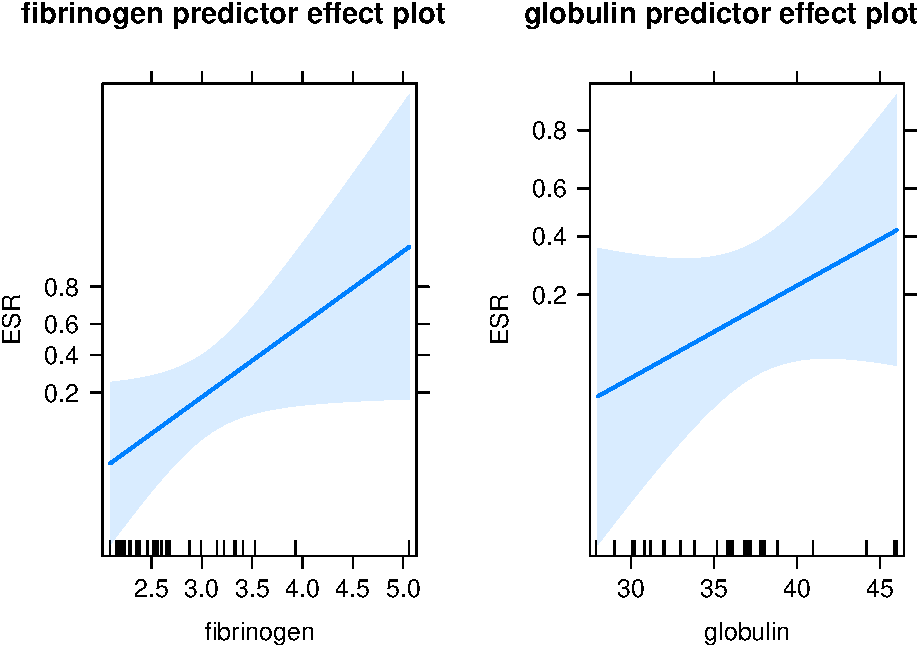
\includegraphics{LogisticRegressionCh5_files/figure-latex/unnamed-chunk-6-2.pdf}

\hypertarget{interpretation-of-regression-coefficients}{%
\subsection{Interpretation of Regression
Coefficients}\label{interpretation-of-regression-coefficients}}

So, the estimated logistic-regression model is given by

\[log[\frac{\hat\mu(x)}{1-\hat\mu(x)}] = \beta_0 + \beta_1 x_1 + \beta_2 x_2 + \cdots + \beta_k x_k\]

If exponentiate both sides of the equation, we get
\[\frac{\hat\mu(x)}{1-\hat\mu(x)} = exp(\beta_0) \times exp(\beta_1 x_1) \times exp(\beta_2 x_2) \times \cdots \times exp(beta_k x_k)\]

where the left hadn of the equation,
\(\frac{\hat\mu(x)}{1-\hat\mu(x)}\), gives the \emph{fitted odds} of
success, \textbf{the fitted probability of success divided by the fitted
probability of failure}. Exponentiating the model removes the logarithms
and vhanges the model in the log-odds scale to one that is
multiplicative, in this log odds scale.

For the WCGS data and the variable Corollary Heart Disease (CHD) and
age, the \(\beta_1\) is the age slope of the fitted logistic model. The
outcome of the model is the log odds of CHD risk and the relationship
with age, the slope coefficient \(\beta_1\) gives the change in the log
odds of chd69 associated with the model.

\begin{Shaded}
\begin{Highlighting}[]
\NormalTok{wcgs <-}\StringTok{ }\KeywordTok{mutate}\NormalTok{(wcgs, }\DataTypeTok{chd69 =} \KeywordTok{factor}\NormalTok{(chd69))}
\CommentTok{# For table 5.2}
\NormalTok{CHD_glm01 <-}\StringTok{ }\KeywordTok{glm}\NormalTok{(chd69 }\OperatorTok{~}\StringTok{ }\NormalTok{age, }\DataTypeTok{data =}\NormalTok{ wcgs, }\DataTypeTok{family =} \KeywordTok{binomial}\NormalTok{())}
\KeywordTok{S}\NormalTok{(CHD_glm01)}
\end{Highlighting}
\end{Shaded}

\begin{verbatim}
Call: glm(formula = chd69 ~ age, family = binomial(), data = wcgs)

Coefficients:
            Estimate Std. Error z value Pr(>|z|)    
(Intercept) -5.93952    0.54932 -10.813  < 2e-16 ***
age          0.07442    0.01130   6.585 4.56e-11 ***
---
Signif. codes:  0 '***' 0.001 '**' 0.01 '*' 0.05 '.' 0.1 ' ' 1

(Dispersion parameter for binomial family taken to be 1)

    Null deviance: 1781.2  on 3153  degrees of freedom
Residual deviance: 1738.4  on 3152  degrees of freedom

 logLik      df     AIC     BIC 
-869.18       2 1742.36 1754.47 

Number of Fisher Scoring iterations: 5

Exponentiated Coefficients and Confidence Bounds
               Estimate        2.5 %      97.5 %
(Intercept) 0.002633304 0.0008898193 0.007676359
age         1.077261913 1.0536638869 1.101432899
\end{verbatim}

\begin{Shaded}
\begin{Highlighting}[]
\CommentTok{#confint(CHD_glm01, parm = "age")}
\CommentTok{# To estimate the model}
\KeywordTok{exp}\NormalTok{(}\KeywordTok{coef}\NormalTok{(CHD_glm01)[}\StringTok{"age"}\NormalTok{])}
\end{Highlighting}
\end{Shaded}

\begin{verbatim}
     age 
1.077262 
\end{verbatim}

The link transformation is the exponentiation, to obtain the odds.

\end{document}
